\documentclass[11pt,a4paper]{article}
\usepackage[T1]{fontenc}
\usepackage[utf8]{inputenc}
\usepackage{lmodern,microtype}
\usepackage[margin=23mm]{geometry}
\usepackage{amsmath,amssymb,booktabs,array,graphicx,siunitx,xurl}
\usepackage[numbers,sort&compress]{natbib}
\usepackage[colorlinks=true,linkcolor=blue!50!black,citecolor=blue!50!black,urlcolor=blue!50!black]{hyperref}
\usepackage{xcolor,placeins}
\graphicspath{{figures/}}
\newcommand{\dd}{\mathrm{d}}
\newcommand{\code}[1]{\path{#1}}
\newcommand{\sinc}{\operatorname{sinc}}
\newcommand{\CD}{C_D}
\newcommand{\Cf}{C_f}
\newcommand{\Tcds}{T_{\rm CDS}}
\newcommand{\Vref}{V_{\rm REF}}
\newcommand{\Voff}{V_{\rm OFF}}
\setlength{\parindent}{0pt}
\setlength{\parskip}{5pt plus 1pt}
\setlength{\emergencystretch}{3em}
\title{Electronic noise\\[4pt]\large Thermal and flicker noise of resistors and MOS transistors}
\author{J.J. Gómez-Cadenas}
\date{14 November 2026}
\begin{document}
\maketitle
\begin{abstract}
A study note on the origin of the three noise spectral densities used in the
analysis of the NAUSICAA charge-sensitive amplifier \citep{HerreroGarcia2026}:
the thermal noise of a resistor, the thermal noise of the channel of a MOS
transistor, and the flicker noise of the same transistor. A short section on
the MOS transistor provides the vocabulary.
\end{abstract}
\tableofcontents

% ----------------------------------------------------------------------
\section{Scope and notation}
\label{sec:scope}
%
This note derives, from the thermal motion of charge, the spectral densities
of the noise sources that the companion note on the NAUSICAA
charge-sensitive amplifier \citep{HerreroGarcia2026} takes as given.
Section~\ref{sec:mosfet} summarises how a MOS transistor works, to the extent
needed. The results are textbook material
\citep{vanderZiel1986,Tsividis2011}.
%
\begin{itemize}
\item A noise voltage $e(t)$ is a random function of time with zero mean.
  Its size is measured by the time average of its square, $\langle
  e^2\rangle$, in \si{V^2}.
\item The spectral density $e^2(f)$, in \si{V^2/Hz}, says how that mean
  square is distributed in frequency: $\langle e^2\rangle=\int_0^\infty
  e^2(f)\,\dd f$. Only positive frequencies are counted. For a current the
  density $i^2(f)$ is in \si{A^2/Hz}.
\item Noise is white when $e^2(f)$ does not depend on $f$, and flicker or
  $1/f$ noise when $e^2(f)\propto1/f$.
\item Independent noise sources with zero mean add in mean square,
  $\langle(a+b)^2\rangle=\langle a^2\rangle+\langle b^2\rangle$, because the
  cross term averages to zero. Their spectral densities add in the same way.
\item A linear filter with transfer function $H(f)$ turns a density
  $e^2(f)$ into $|H(f)|^2\,e^2(f)$.
\item $k$ is Boltzmann's constant and $T_{\rm K}$ the absolute temperature;
  $4kT_{\rm K}=\SI{1.66e-20}{J}$ at \SI{300}{K}.
\end{itemize}

% ----------------------------------------------------------------------
\section{The MOS transistor}
\label{sec:mosfet}
%
\begin{figure}[htbp]\centering
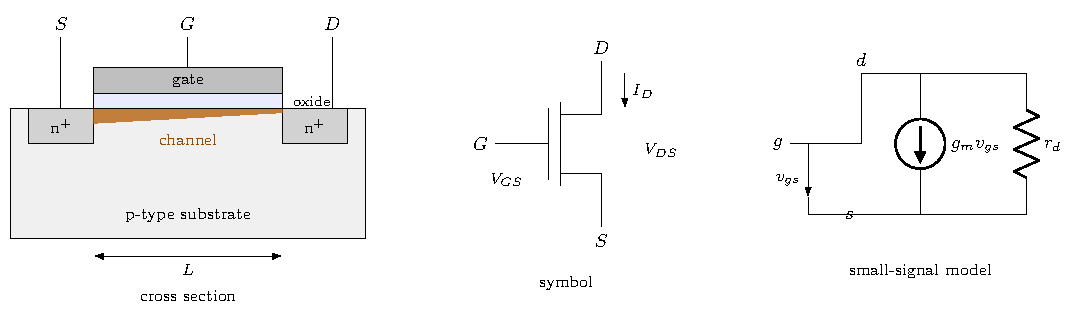
\includegraphics[width=\linewidth]{electronic_noise_mosfet.pdf}
\caption{An n-channel MOS transistor. Left: cross section, with the source
and drain regions, the gate above the oxide, and the channel of mobile
electrons induced under the oxide. Centre: circuit symbol and the voltages
and current used in the text. Right: small-signal model, a current source
$g_mv_{gs}$ between drain and source with the output resistance $r_d$ in
parallel.}
\label{fig:mosfet}
\end{figure}
%
Figure~\ref{fig:mosfet} shows an n-channel MOS transistor. Two heavily doped
n-type regions, the source and the drain, are implanted in a p-type silicon
substrate. Between them a thin oxide layer separates the substrate from the
gate, a conducting electrode. Gate, oxide and substrate form a capacitor with
capacitance $C_{\rm ox}$ per unit area. The channel has length $L$ from
source to drain and width $W$ across the page.

\paragraph{Channel.} With the gate at the potential of the source, the two
n-type regions are separated by the substrate and no current flows between
them. A positive gate voltage attracts electrons to the surface of the
substrate under the oxide. Above a threshold $V_T$ a thin layer of mobile
electrons, the channel, connects source and drain. As on any capacitor, the
mobile charge per unit area is the capacitance times the voltage in excess
of the threshold. At a point where the channel is at potential $V$ with
respect to the source, the voltage between gate and channel is $V_{GS}-V$
and the charge per unit length is
%
\[
 |Q'| = WC_{\rm ox}\,(V_{GS}-V_T-V) = WC_{\rm ox}\,(V_{\rm ov}-V),
 \qquad V_{\rm ov}=V_{GS}-V_T ,
\]
%
where $V_{\rm ov}$ is the gate voltage above threshold. No current flows
through the oxide: the gate controls the channel without drawing current.

\paragraph{Current.} A voltage $V_{DS}$ between drain and source makes the
electrons drift along the channel with velocity $\mu\,\dd V/\dd x$, where
$\mu$ is their mobility and $x$ the position along the channel, so the
current is $I_D=\mu|Q'|\,\dd V/\dd x$, the same at every point. Integrating
from the source, where $V=0$, to the drain, where $V=V_{DS}$
(Section~\ref{sec:channel} does this step by step),
%
\[
 I_D = \frac{\mu WC_{\rm ox}}{L}\left[V_{\rm ov}V_{DS}-\frac{V_{DS}^2}{2}\right],
 \qquad V_{DS}\le V_{\rm ov} .
\]
%
For small $V_{DS}$ the current is proportional to $V_{DS}$: the transistor is
a resistor of value $L/(\mu WC_{\rm ox}V_{\rm ov})$, controlled by the gate.
As $V_{DS}$ grows, the charge at the drain end, $WC_{\rm ox}(V_{\rm
ov}-V_{DS})$, shrinks. At $V_{DS}=V_{\rm ov}$ it is zero and the current
reaches
%
\[
 I_D = \frac{\mu WC_{\rm ox}}{2L}\,V_{\rm ov}^2 ,
\]
%
beyond which it no longer depends on $V_{DS}$. This regime, called
saturation, is where a transistor amplifies: the drain current is set by the
gate voltage alone. Below threshold a small current remains, carried by
diffusion and exponential in $V_{GS}$. This is the weak-inversion regime, in
which the feedback transistor of the present NAUSICAA amplifier operates.

\paragraph{Small signals.} An amplifier applies a small variation $v_{gs}$
of the gate voltage around a fixed operating point and uses the resulting
variation $i_d$ of the drain current. For small variations the relation is
linear,
%
\[
 i_d = g_m\,v_{gs} + \frac{v_{ds}}{r_d},
 \qquad
 g_m=\frac{\partial I_D}{\partial V_{GS}}=\frac{\mu WC_{\rm ox}}{L}\,V_{\rm ov},
 \qquad
 \frac{1}{r_d}=\frac{\partial I_D}{\partial V_{DS}} .
\]
%
The transconductance $g_m$ is the change of drain current per change of gate
voltage: the transistor is a voltage-controlled current source
(Fig.~\ref{fig:mosfet}, right). It equals the conductance of the channel at
small $V_{DS}$, which is why the channel is said to be a resistor of value
$1/g_m$. The output resistance $r_d$ expresses the small residual dependence
of the current on $V_{DS}$ in saturation; it is large. With a load of
impedance $Z_L$ at the drain and $r_d\gg Z_L$, the drain voltage changes by
$-g_mZ_Lv_{gs}$: this is the voltage gain of a single transistor stage, and
the origin of the factors $g_mr_d$ in the cascode analysis of the companion
note.

A p-channel transistor is the same device with the doping reversed: the
channel is made of holes and all voltages and currents change sign. In an
amplifier the p-channel transistors serve as loads and current sources for
the n-channel stages.

%

% ----------------------------------------------------------------------

% ----------------------------------------------------------------------
\section{Thermal noise of a resistor}
\label{sec:resistor}
%
\begin{figure}[htbp]\centering
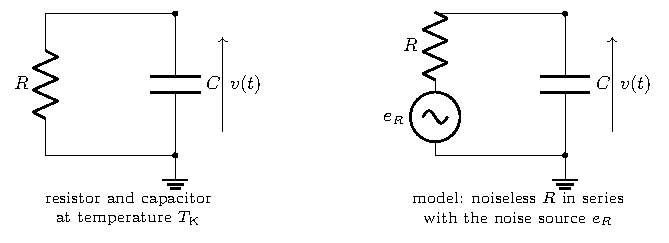
\includegraphics[width=.7\linewidth]{nausicaa_vh_rc.pdf}
\caption{Left: a resistor and a capacitor in parallel, in thermal
equilibrium; $v(t)$ is the voltage across both. Right: the same pair with
the thermal agitation of the resistor represented by a voltage source $e_R$
in series with a noiseless resistor.}
\label{fig:rc}
\end{figure}
%
Consider a resistor $R$ connected to a capacitor $C$ in thermal
equilibrium at temperature $T_{\rm K}$ (Fig.~\ref{fig:rc}, left). Let $v(t)$
be the voltage across the capacitor (resistor). Due to thermal agitation of the
charge carriers in the resistor, $v(t)$ fluctuates in time. The capacitor
stores the energy $Cv^2/2$. By equipartition,
%
\begin{equation}
 \tfrac12\, C\,\langle v^2\rangle = \tfrac12\, kT_{\rm K}
 \quad\Longrightarrow\quad
 \langle v^2\rangle = \frac{kT_{\rm K}}{C} ,
\label{eq:ktc}
\end{equation}
%
where $\langle v^2\rangle$ is the time average of $v^2(t)$ and $k$ is
Boltzmann's constant.

We can model the resistor noise as a noiseless resistor in series with a voltage source
$e_R$ with constant spectral density $e_R^2$ at every frequency, i.e.\ white
noise (Fig.~\ref{fig:rc}, right). The capacitor voltage is obtained from $e_R$ filtered
by the $RC$ low pass,
$|H(f)|^2=1/[1+(2\pi fRC)^2]$:
%
\begin{equation}
 \langle v^2\rangle = e_R^2\int_0^\infty\frac{\dd f}{1+(2\pi fRC)^2}
 = \frac{e_R^2}{4RC} .
\end{equation}
%
Equating the two expressions for $\langle v^2\rangle$ we obtain the Nyquist
formula \citep{Nyquist1928,Johnson1928},
%
\begin{equation}
 \boxed{\; e_R^2 = 4kT_{\rm K}R \;}
 \qquad\text{or, as a current source in parallel,}\qquad
 \boxed{\; i_R^2 = \frac{e_R^2}{R^2} = \frac{4kT_{\rm K}}{R} \;} .
\label{eq:nyquist}
\end{equation}
%

% ----------------------------------------------------------------------
\section{Thermal noise of a transistor channel}
\label{sec:channel}
%
\begin{figure}[htbp]\centering
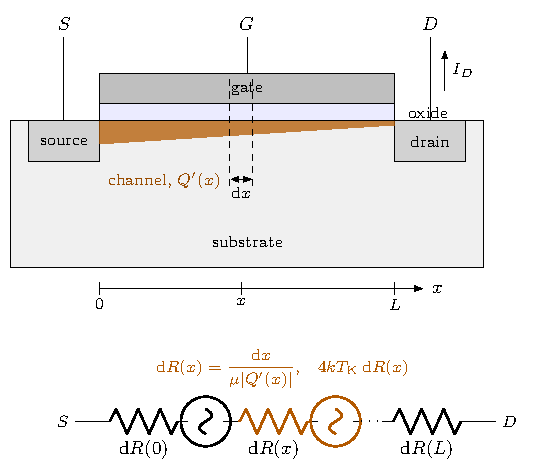
\includegraphics[width=.50\linewidth]{nausicaa_vh_channel.pdf}
\caption{Top: cross section of a MOS transistor in saturation. The channel
is the layer of mobile charge under the oxide, from the source at $x=0$ to
the drain at $x=L$; its charge per unit length $Q'(x)$ decreases from the
source to the drain. Bottom: the channel as a series chain of segments of length $\dd x$,
each a resistor $\dd R(x)$ with its own thermal noise source.}
\label{fig:channel}
\end{figure}
%
The channel of a MOS
transistor is a thin layer of mobile charge under the gate oxide, from the
source at $x=0$ to the drain at $x=L$ (Figure~\ref{fig:channel}). Call $Q'(x)$ the charge per unit
length, $\mu$ the carrier mobility and $V(x)$ the potential
along the channel. The noise of the channel is computed as follows:
%
\begin{itemize}
\item \textbf{The drain current} $I_D$ is the charge per
  unit length times the drift velocity $\mu\,\dd V/\dd x$,
%
  \[
   I_D = \mu\,|Q'(x)|\,\frac{\dd V}{\dd x} .
  \]
%
\item \textbf{A segment of length $\dd x$ drops a voltage} $\dd V$,
%
  \[
   \dd V = \frac{I_D\,\dd x}{\mu\,|Q'(x)|} .
  \]
%
\item \textbf{The resistance of a segment} $\dd R(x)$ is therefore
%
  \[
   \dd R(x) = \frac{\dd V}{I_D} = \frac{\dd x}{\mu\,|Q'(x)|} .
  \]
%
  The channel is the series connection of these segments
  (Fig.~\ref{fig:channel}, bottom).
\item \textbf{Noise of a segment.} Each segment is a resistor in thermal
  equilibrium, and Eq.~\eqref{eq:nyquist} gives its noise voltage, in series
  with it,
%
  \[
   \dd e^2 = 4kT_{\rm K}\,\dd R(x) = \frac{4kT_{\rm K}\,\dd x}{\mu\,|Q'(x)|} .
  \]
%
\item \textbf{From the noise voltage of a segment to the drain current.}
  To compute the effect of the noise voltage in the drain current, we consider the
  the change of drain current produced by a
  diferential voltage $\delta v$ placed in series with the channel at the position
  of the segment, $\delta I_D/\delta v$. Using the fact that the circuit is linear for small signals, $\delta I_D/\delta v$ converts the random noise voltage of that segment into drain
  current. Since $I_D$ is the same at every $x$: 
  %Integrating
  %$I_D\,\dd x=\mu|Q'(x)|\,\dd V$ along the channel, where $V$ runs from
  %$0$ at the source to $V_{DS}$ at the drain,
%
  \[
  \int I_D\,\dd x =
   I_D\,L = \int \mu|Q'(x)|\,\dd V = \mu\int_0^{V_{DS}}|Q'(V)|\,\dd V .
  \]
%
  Figure~\ref{fig:testvoltage} shows the construction. Add a small
  voltage source $\delta v$ to the chain of segments at the point $x_0$,  keeping the
  source at $0$ and the drain at $V_{DS}$. $V_0$ is the
  potential before the source and 
  $V_0+\delta v$ the potential right after. The same current $I'$ flows in the segments before and
  after the added source, because the channel is its only path. The bottom
  panel shows the potential along the channel with and without $\delta v$:
  the two agree up to $x_0$, differ by $\delta v$ just after it, and both
  reach $V_{DS}$ at the drain. Now integrate $I'\,\dd x=\mu|Q'|\,\dd V$
  over the three parts of the chain.
%
  \begin{figure}[htbp]\centering
  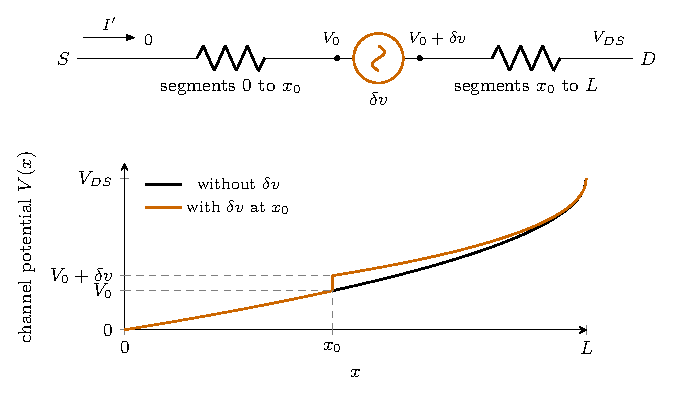
\includegraphics[width=.6\linewidth]{nausicaa_vh_testvoltage.pdf}
  \caption{Top: the chain of channel segments with a small voltage source
  $\delta v$ added at $x_0$; the potentials at the ends of the two groups of
  segments are marked. Bottom: potential along the channel without the added
  source (black) and with it (orange).}
  \label{fig:testvoltage}
  \end{figure}
%
  \begin{itemize}
  \item Before the added source, over the segments from $x=0$ to $x=x_0$,
    where the potential goes from $0$ to $V_0$:
%
    \[
     \int_0^{x_0} I'\,\dd x = I'\,x_0
     = \mu\int_0^{V_0}|Q'(V)|\,\dd V .
    \]
%
  \item Across the added source the potential rises from $V_0$ to
    $V_0+\delta v$.
  \item After the added source, over the segments from $x=x_0$ to $x=L$,
    where the potential goes from $V_0+\delta v$ to $V_{DS}$:
%
    \[
     \int_{x_0}^{L} I'\,\dd x = I'\,(L-x_0)
     = \mu\int_{V_0+\delta v}^{V_{DS}}|Q'(V)|\,\dd V .
    \]
%
  \end{itemize}
%
  Adding the three lines, and splitting the range $0$ to $V_{DS}$ of the
  channel without the added source into the same three pieces,
%
  \begin{align*}
   I'\,L &= \mu\int_0^{V_0}|Q'(V)|\,\dd V
         + \mu\int_{V_0+\delta v}^{V_{DS}}|Q'(V)|\,\dd V ,\\
   I_D\,L &= \mu\int_0^{V_{DS}}|Q'(V)|\,\dd V
         = \mu\int_0^{V_0}|Q'(V)|\,\dd V
         + \mu\int_{V_0}^{V_0+\delta v}|Q'(V)|\,\dd V
         + \mu\int_{V_0+\delta v}^{V_{DS}}|Q'(V)|\,\dd V .
  \end{align*}
%
  Subtracting the first line from the second,
%
  \[
   (I_D-I')\,L = \mu\int_{V_0}^{V_0+\delta v}|Q'(V)|\,\dd V
   = \mu\,|Q'(V_0)|\,\delta v
   = \mu\,|Q'(x_0)|\,\delta v ,
  \]
%
  since over an interval of width $\delta v$ the integrand is constant and
  $V_0=V(x_0)$. The position $x_0$ has dropped out, and the drain current
  changes by
%
  \[
   \delta I_D = I'-I_D = -\frac{\mu\,|Q'(x_0)|}{L}\,\delta v
  \]
%
  \citep{Tsividis2011}. The sign says which way the current moves for a
  given polarity of $\delta v$ and does not matter for noise. The ratio depends on the position: a segment
  near the drain, where the charge is small, has a large noise voltage but
  converts it into drain current with a small factor.
\item \textbf{Sum over the channel.} The segment at $x$ contributes to
  the drain current a fluctuation whose mean square is
  $(\delta I_D/\delta v)^2\,\dd e^2$. The noise voltages of different
  segments are independent and have zero mean, so when their contributions
  are added the cross terms average to zero and the mean square of the total
  is the sum of the mean squares:
%
\begin{equation}
 i_d^2=\int_0^L\left(\frac{\mu|Q'(x)|}{L}\right)^2
 \frac{4kT_{\rm K}\,\dd x}{\mu|Q'(x)|}
 =\frac{4kT_{\rm K}\,\mu}{L^2}\,|Q_{\rm inv}| ,
 \qquad Q_{\rm inv}=\int_0^L Q'(x)\,\dd x .
\label{eq:idsq}
\end{equation}
%
  %The product of a large $\dd R$ and a small conversion factor scales as
  %$|Q'(x)|$: the segments with more charge contribute more.
\end{itemize}
%
The channel noise is thus the thermal noise of a conductance
$\mu|Q_{\rm inv}|/L^2$, set by the total charge in the channel.

To evaluate $|Q_{\rm inv}|$ the charge profile along the channel is
needed. It follows from how the gate controls the channel.
%
\begin{itemize}
\item \textbf{Charge induced by the gate.} The gate, the oxide and the
  channel form a capacitor of capacitance $C_{\rm ox}$ per unit area. Below
  a threshold gate voltage $V_T$ the channel holds no mobile charge; above
  it, the mobile charge per unit area is $C_{\rm ox}$ times the voltage in
  excess of the threshold, as on any capacitor. At the point $x$ the channel
  is at the potential $V(x)$, so the voltage between gate and channel there
  is $V_{GS}-V(x)$ and the charge per unit length, for a channel of width
  $W$, is
%
  \[
   |Q'(x)| = W\,C_{\rm ox}\,[\,V_{\rm ov}-V(x)\,],
   \qquad V_{\rm ov} = V_{GS}-V_T ,
  \]
%
  where $V_{\rm ov}$ is the gate voltage above threshold. The charge is
  largest at the source, $WC_{\rm ox}V_{\rm ov}$ at $V=0$, and decreases
  towards the drain as the channel potential rises.
\item \textbf{Saturation.} When the drain is so positive that the channel
  potential at its end reaches $V_{\rm ov}$, the charge there is zero and
  the current no longer grows with $V_{DS}$. This is the normal operating
  regime of an amplifying transistor. The channel potential then runs from
  $0$ at the source to $V_{\rm ov}$ at the drain, and the current relation
  of the previous step gives
%
  \[
   I_D\,L = \mu\int_0^{V_{\rm ov}} WC_{\rm ox}\,(V_{\rm ov}-V)\,\dd V
          = \frac{\mu WC_{\rm ox}V_{\rm ov}^2}{2}
   \quad\Longrightarrow\quad
   I_D = \frac{\mu WC_{\rm ox}}{2L}\,V_{\rm ov}^2 .
  \]
%
\item \textbf{Total channel charge.} $Q_{\rm inv}=\int_0^L Q'(x)\,\dd x$
  is converted to an integral over the potential with
  $\dd x=\mu|Q'|\,\dd V/I_D$, from the current relation:
%
  \begin{align*}
   |Q_{\rm inv}| &= \frac{\mu}{I_D}\int_0^{V_{\rm ov}}|Q'(V)|^2\,\dd V
   = \frac{\mu}{I_D}\,(WC_{\rm ox})^2\int_0^{V_{\rm ov}}(V_{\rm ov}-V)^2\,\dd V \\
   &= \frac{\mu(WC_{\rm ox})^2V_{\rm ov}^3}{3\,I_D}
   = \frac23\,WLC_{\rm ox}V_{\rm ov} ,
  \end{align*}
%
  using the expression of $I_D$ in the last step. The average charge per
  unit length is two thirds of its value at the source.
\item \textbf{Transconductance.} The transconductance $g_m$ is the change
  of drain current per change of gate voltage, the quantity that converts
  a voltage at the gate into a current at the drain. From the expression of
  $I_D$, with $\partial V_{\rm ov}/\partial V_{GS}=1$,
%
  \[
   g_m = \frac{\partial I_D}{\partial V_{GS}}
       = \frac{\mu WC_{\rm ox}}{L}\,V_{\rm ov} .
  \]
%
\end{itemize}
%
Inserting $|Q_{\rm inv}|$ in Eq.~\eqref{eq:idsq}, the product
$\mu WC_{\rm ox}V_{\rm ov}/L$ that appears is the transconductance of
the last step:
%
\begin{equation}
 i_d^2=\frac{4kT_{\rm K}\,\mu}{L^2}\cdot\frac23\,WLC_{\rm ox}V_{\rm ov}
 =\frac23\,4kT_{\rm K}\,\frac{\mu WC_{\rm ox}V_{\rm ov}}{L}
 =\frac23\,4kT_{\rm K}\,g_m .
\label{eq:iddrain}
\end{equation}
%
The factor $2/3$ is the long-channel value of $\gamma$. The conductance of
the channel with uniform charge, at $V_{DS}=0$ where $|Q'|=WC_{\rm ox}V_{\rm ov}$
everywhere, is $\mu WC_{\rm ox}V_{\rm ov}/L=g_m$: this is the sense in which
the channel is a resistor of value $1/g_m$, and $\gamma$ is the correction for
the charge lost towards the drain in saturation. In short channels, velocity
saturation and carrier heating raise $\gamma$ to about $1$; in weak
inversion the current is a shot-noise-like diffusion current and
$\gamma$ lies between $1/2$ and $2/3$ \citep{vanderZiel1986,Tsividis2011}.

The drain-current noise is referred to the gate by asking which gate voltage
would produce it. A gate fluctuation $e_g$ gives a drain current $g_m e_g$,
so $i_d^2=g_m^2e_g^2$ and
%
\begin{equation}
 \boxed{\; e_t^2=\frac{i_d^2}{g_m^2}=\frac{4kT_{\rm K}\,\gamma}{g_m} \;}.
\label{eq:et}
\end{equation}
%
Compared with Eq.~\eqref{eq:nyquist}, the transistor behaves as if a
resistor $\gamma/g_m$ sat in series with its gate. A transconductance of
\SI{1}{mS} corresponds to \SI{700}{\ohm} and a noise density of
\SI{3.4}{nV/\sqrt{Hz}} at room temperature. Since $g_m$ grows with the drain
current and with $W/L$, the input transistor of a low-noise front end is
given most of the current budget of the amplifier and a wide channel.

% ----------------------------------------------------------------------
\section{Flicker noise}
\label{sec:flicker}
%
The gate oxide contains traps within tunnelling distance of the channel. A
trap captures a channel carrier and releases it after a random time; while
the carrier is trapped the channel has one carrier less and its charge is
displaced by $e$. One trap with mean capture and release time $\tau$
produces a random telegraph signal whose spectrum is a Lorentzian,
$S(f)\propto\tau/[1+(2\pi f\tau)^2]$: flat below $1/(2\pi\tau)$ and falling
as $1/f^2$ above. The tunnelling probability falls exponentially with the
depth $z$ of the trap in the oxide, so $\tau\propto\exp(z/\lambda)$ with
$\lambda$ of order \SI{0.1}{nm}. Traps distributed uniformly in $z$ are
therefore distributed uniformly in $\ln\tau$, with density proportional to
$1/\tau$ in $\tau$. Summing their Lorentzians,
%
\begin{equation}
 S(f)\propto\int_{\tau_1}^{\tau_2}\frac{1}{\tau}\,
 \frac{\tau\,\dd\tau}{1+(2\pi f\tau)^2}
 =\frac{1}{2\pi f}\left[\arctan(2\pi f\tau_2)-\arctan(2\pi f\tau_1)\right]
 \simeq\frac{1}{4f}
\label{eq:lorentzsum}
\end{equation}
%
for $1/\tau_2\ll 2\pi f\ll 1/\tau_1$: the superposition of time constants
spread over many decades is a $1/f$ spectrum over those decades
\citep{McWhorter1957}. Each trapping event shifts the channel charge by one
$e$, which is equivalent to a gate voltage step $e/(WLC_{\rm ox})$; the
number of active traps grows with the gate area $WL$. The spectral density
referred to the gate is therefore
%
\begin{equation}
 \boxed{\; e_f^2=\frac{A_f}{f},\qquad
 A_f=\frac{K_f}{C_{\rm ox}^2\,WL} \;},
\label{eq:af}
\end{equation}
%
where $K_f$ collects the trap density and the tunnelling parameters of the
technology \citep{Tsividis2011}. Flicker noise falls with gate area, thermal
noise falls with $g_m$. The input transistor is made large for the first
reason and wide for the second, and the corner frequency $f_c=A_f/e_t^2$
measures how well the two have been balanced.

\bibliographystyle{unsrtnat}
\bibliography{references}
\end{document}
